\section{Cooperative Middleware Platform as a Service}
\label{sec:COMPaaS}
Cooperative Middleware Platform as a Service (COMPaaS) é um sistema que provê aos usuários uma simples e bem
definida plataforma de serviços para o desenvolvimento de aplicações de \textit{Internet of Things}.

O COMPaaS amplia as especificações do EPCglobal em relação às interfaces de middleware RFID para
prover serviços de alto nível. Além disso, provê também uma leve arquitetura baseada nas especificações
ETSI para plataforma de serviços M2M, assim como uma aplicação web para integração de dispositivos físicos.
O intuito principal desta plataforma se estende desde o gerenciamento de dados até a integração dos
dispositivos, provendo uma serviços cooperativos e de alto nível para as aplicações~\cite{COMPaaS}.

Ele é composto por 3 subsistemas, a saber:  Application Level Events
Interface (ALE), Middleware Level Events Interface (MLE) e Device Level Protocol (DLE).

\begin{figure}[H]
	\centering
		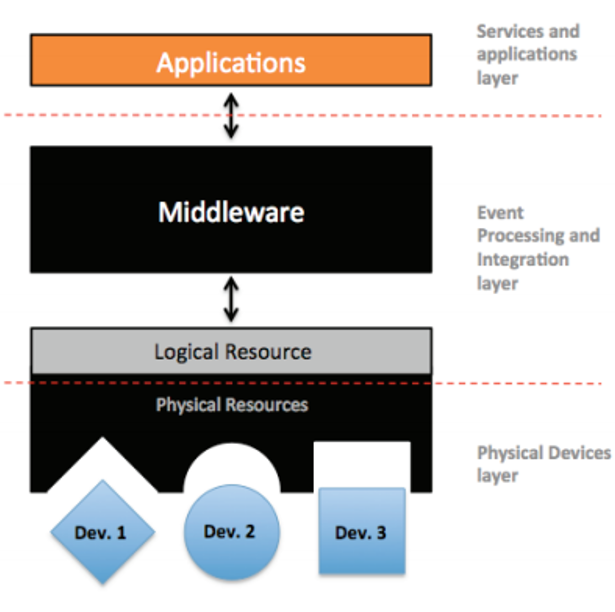
\includegraphics[width=0.5\textwidth]{fig/compaas_arch.png}
	\caption{Arquitetura em alto nível do COMPaaS.}
\end{figure}

\subsection{Application Level Events Interface}
O \textit{Application Level Events} (ALE) expõe uma interface SOAP para a comunicação com as aplicações.
Ele é responsável por receber as requisições das aplicações e encaminha-las ao MLE. As informações
requisitadas são recebidas do MLE por meio de um WebSocket.

\subsection{Middleware Level Events Interface}
O MLE expõe uma interface RESTful para a comunicação com o ALE. É responsável pelo recebimento das requisições
oriundas do ALE para então encaminhar as mesma para o DLE. Os dados retornados do DLE, no formato de DataMessage
object, são então enviados ao ALE por meio de WebSocket.

\subsection{Device Level Events}
O DLE cria um dispositivo virtual em torno do dispositivo físico e é responsável por definir o formato do DataMessage
object e expor as funcionalidades que são realizadas pelo dispositivo físico. O DLE é o responsável por saber das
minúcias de cada dispositivo, então, para cada novo dispositivo que se deseja incluir na IoT, é necessário criar
um DLE específico para aquele dispositivo. Isto é um pouco oneroso e será um dos temas abordados neste trabalho.
